\section*{Chapter 3}

\subsection*{Exercise 3.1}

\begin{enumerate}
    \item 
    \begin{minipage}[t]{0.45\linewidth}
        At $k = 2$, 
        $\begin{aligned}[t]
            4x^2 + y^2 + 1 &= 2 \\
            4x^2 + y^2     &= 1 \\
            \left(\frac{x}{\frac{1}{2}}\right)^2 + \left(\frac{y}{1}\right)^2 &= 1
        \end{aligned}$
    \end{minipage}
    \begin{minipage}[t]{0.45\linewidth}
        At $k = 5$, 
        $\begin{aligned}[t]
            4x^2 + y^2 + 1      &= 5 \\
            4x^2 + y^2          &= 4 \\
            x^2 + \frac{y^2}{4} &= 1 \\
            \left(\frac{x}{1}\right)^2 + \left(\frac{y}{2}\right)^2 &= 1
        \end{aligned}$
    \end{minipage}

    \begin{center}
        \tikzsetnextfilename{c03e01-01}%
        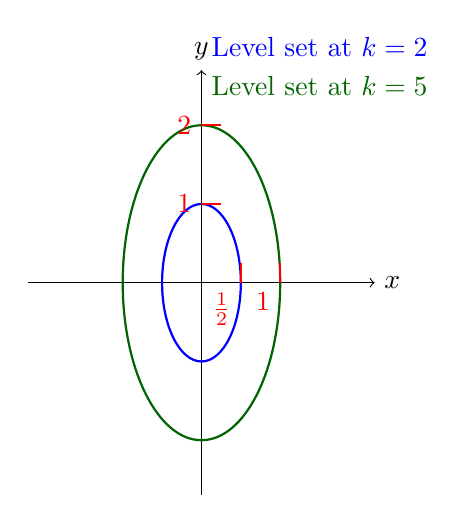
\begin{tikzpicture}
            \draw[->] (-2.2,0) -- (2.2,0) node[right] {$x$};
            \draw[->] (0,-2.7) -- (0,2.7) node[above] {$y$};
            
            \draw[thick,blue] (0,0) ellipse (0.5cm and 1cm);
            \draw[thick,DarkGreen] (0,0) ellipse (1cm and 2cm);

            \draw[thick,red] (0.5,0.25) -- (0.5,0) node[below left] {$\frac{1}{2}$};
            \draw[thick,red] (1,0.25) -- (1,0) node[below left] {$1$};

            \draw[thick,red] (0.25,1) -- (0,1) node[left] {$1$};
            \draw[thick,red] (0.25,2) -- (0,2) node[left] {$2$};

            \node[blue] at (1.5,3) {Level set at $k = 2$};
            \node[DarkGreen] at (1.5,2.5) {Level set at $k = 5$};
        \end{tikzpicture}
    \end{center}

    \item 
    \begin{minipage}[t]{0.45\linewidth}
        At $k = 0$, 
        $\begin{aligned}[t]
            x^2 + y^2 - z &= 0 \\
            x^2 + y^2     &= z \\
            r^2           &= z
        \end{aligned}$
        
        \begin{center} 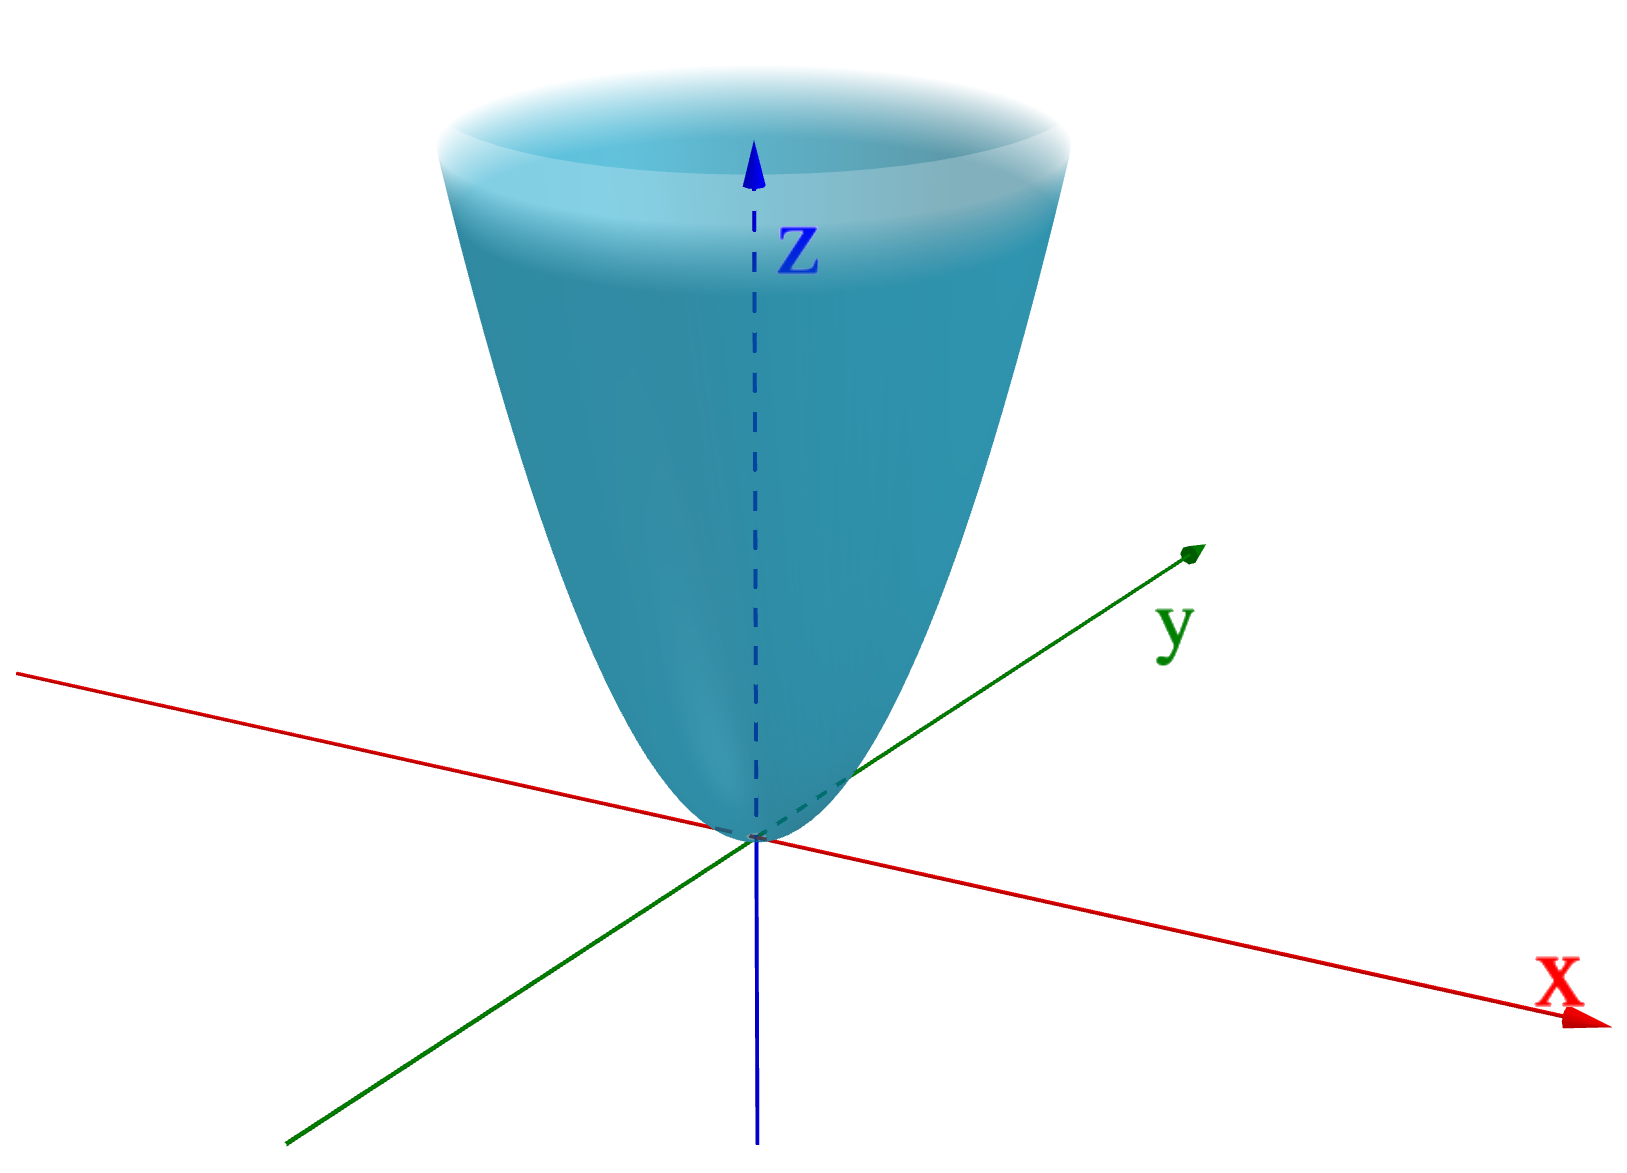
\includegraphics[width=\linewidth]{Plots/e_1_7/1.png} \end{center}
    \end{minipage}
    \begin{minipage}[t]{0.45\linewidth}
        At $k = 2$, 
        $\begin{aligned}[t]
            x^2 + y^2 - z &= 2 \\
            x^2 + y^2 - 2 &= z \\
            r^2 - 2       &= z
        \end{aligned}$

        \begin{center} 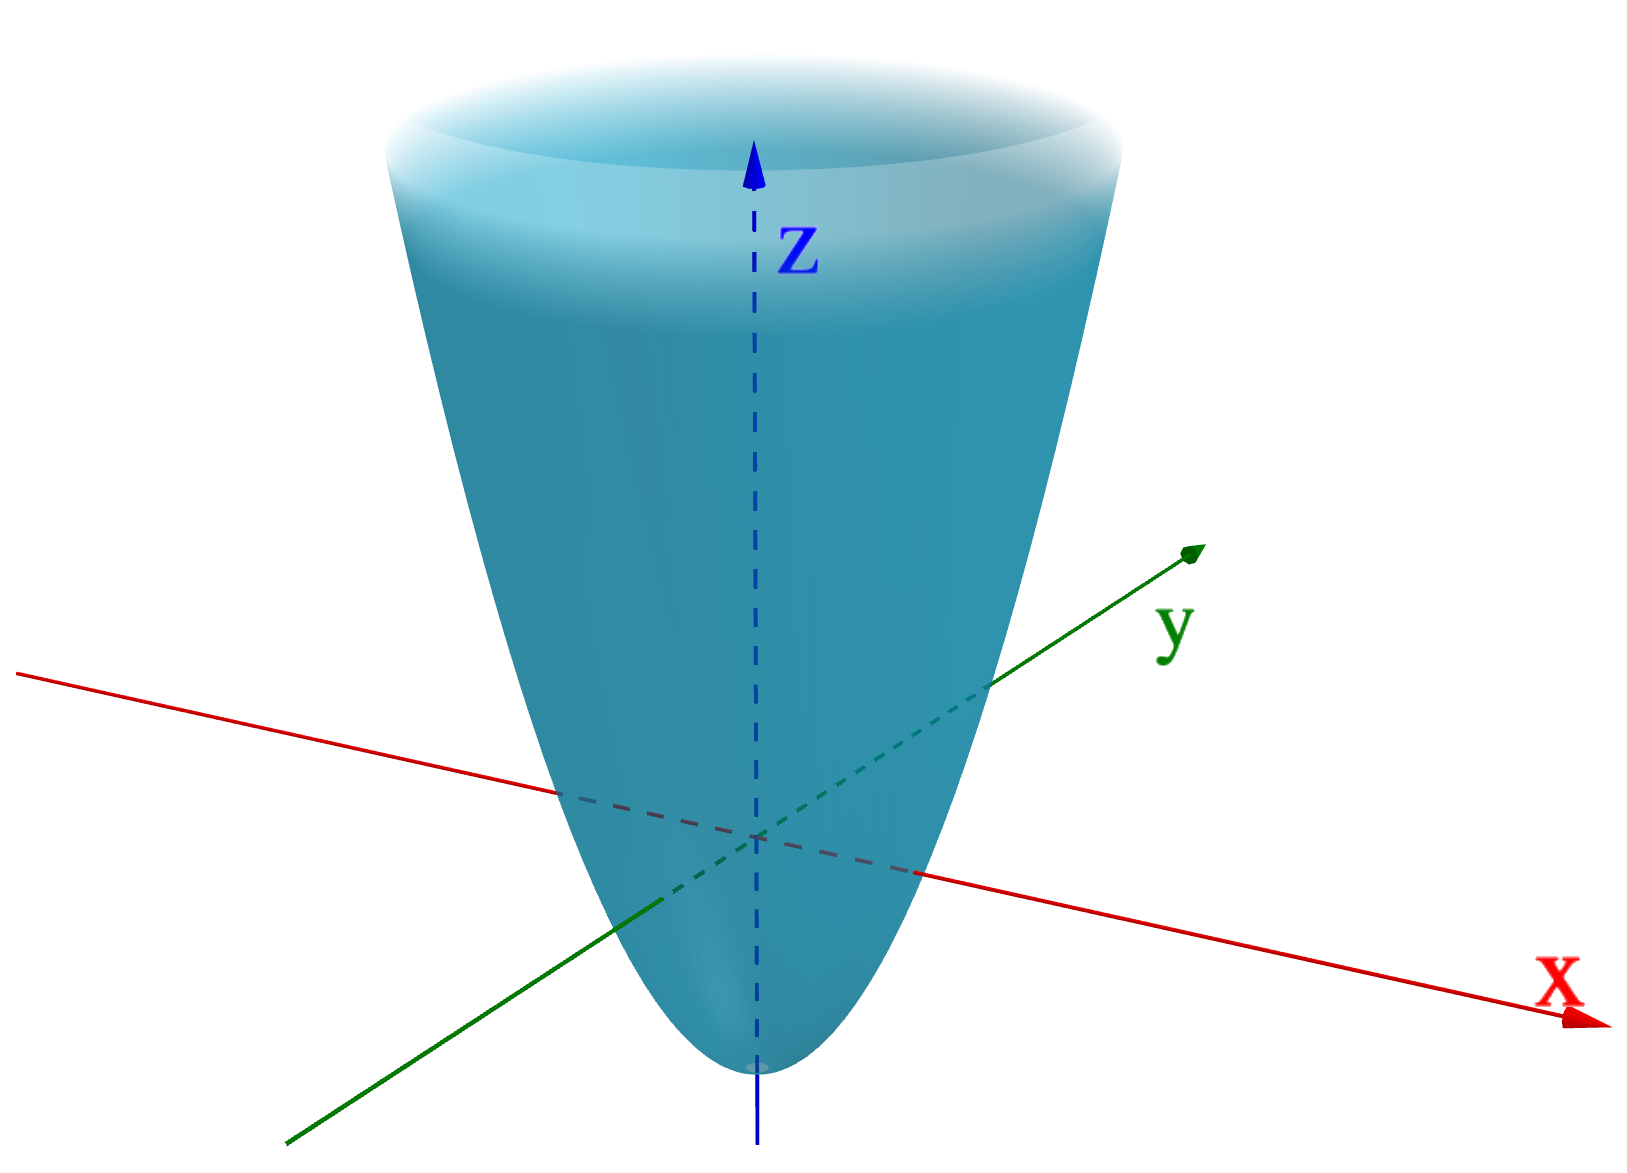
\includegraphics[width=\linewidth]{Plots/e_1_7/2.png} \end{center}
    \end{minipage}
\end{enumerate}

\subsection*{Exercise 3.2}

\begin{itemize}
        \item For $x = 0$, $\lim_{(x,y)\to(0,0)}f(x,y) = \lim_{y\to0}\frac{0}{0 + y^2} = 0$. 

        {~~~}

        \item For $y = x$, $\lim_{(x,y)\to(0,0)}f(x,y) = \lim_{x\to0} \frac{x^2x}{x^4 + x^2} = \lim_{x\to0} \frac{x}{x+1} = 0$. 

        {~~~}

        \item For $y = 0$, $\lim_{(x,y)\to(0,0)}f(x,y) = \lim_{x\to0}\frac{0}{x^4 + 0} = 0$. 

        {~~~}

        \item For $y = x^2$, $\lim_{(x,y)\to(0,0)}f(x,y) = \lim_{x\to0} \frac{x^2x^2}{x^4 + (x^2)^2} = \lim_{x\to0} \frac{x^4}{2x^4} = \frac{1}{2}$. 
\end{itemize} 

Thus, the limit at $(a,y) = (0,0)$ does not exist. 

\subsection*{Exercise 3.3}

$$|f(x, y)| = \left| \frac{xy}{\sqrt{x^4 + y^2}} \right| \le \left| \frac{xy}{\sqrt{y^2}} \right| = \left| \frac{xy}{y} \right| = |x| \to 0$$

Thus, by the Squeeze Theorem, $\lim_{(x,y) \to (0,0)} \frac{xy}{\sqrt{x^4 + y^2}} = 0 = f(0, 0)$. 

Thus, the function is continuous at $(0, 0)$. 

\subsection*{Exercise 3.4}

By removing $2x^4$ from the denominator, we obtain $\left| \frac{x^2 \sin^2{y}}{2x^4 + y^2} \right| \le \left| \frac{x^2 \sin^2{y}}{y^2} \right|$. 

{~~~}

Note that $| \sin{\theta} | \le | \theta |$, and that as $\theta \to 0$, $\sin \theta \approx \theta$. This is the \term{small angle approximation}. 

\begin{center}
    \tikzsetnextfilename{c03e04-01}%
    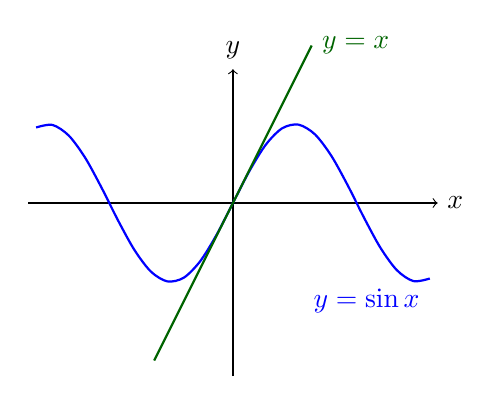
\begin{tikzpicture}
        \draw[->] (-2.6, 0) -- (2.6, 0) node[right] {$x$};
        \draw[->] (0, -2.2) -- (0, 1.7) node[above] {$y$};

        \draw[thick,blue,domain=-2.5:2.5,smooth] plot (\x, {sin(2*\x r)}) node[below left] {$y = \sin{x}$};
        \draw[thick,DarkGreen,domain=-1:1] plot (\x, {2*\x}) node[right] {$y = x$};
    \end{tikzpicture}
\end{center}

So $\left| \frac{x^2 \sin^2{y}}{y^2} \right| \approx \left| \frac{x^2 \cdot y^2}{y^2} \right| = \left| x^2 \right| \to 0$. 

{~~~}

Then, by the Squeeze Theorem, $\lim_{(x,y) \to (0,0)} \frac{x^2 \sin^2{y}}{2x^4 + y^2} = 0$. 

\subsection*{Exercise 3.5}

\begin{enumerate}
    \item 
    $\frac{\partial f}{\partial x} = 2x(y + 1)$ and 
    $\frac{\partial f}{\partial y} = x^2 - 1$. 
    
    So $\nabla f = \left( \frac{\partial f}{\partial x}, \frac{\partial f}{\partial y} \right) = (2x(y + 1), x^2 - 1)$. 

    {~~~}

    \item 
    $\frac{\partial f}{\partial x} = 2{\color{red}y}(xy - 2)$ and 
    $\frac{\partial f}{\partial y} = 2{\color{red}x}(xy - 2)$. 
    
    So $\nabla f = \left( \frac{\partial f}{\partial x}, \frac{\partial f}{\partial y} \right) = (2y(xy - 2), 2x(xy - 2))$. 

    {~~~}

    \item 
    $\frac{\partial f}{\partial x} = \frac{-2}{(x + 3y)^2}$ and 
    $\frac{\partial f}{\partial y} = \frac{-6}{(x + 3y)^2}$. 
    
    So $\nabla f = \left( \frac{\partial f}{\partial x}, \frac{\partial f}{\partial y} \right) = \left( \frac{-2}{(x + 3y)^2}, \frac{-6}{(x + 3y)^2} \right)$. 

    {~~~}

    \item 
    $\frac{\partial f}{\partial x} = e^{x + 4y}$ and 
    $\frac{\partial f}{\partial y} = 4e^{x + 4y}$. 
    
    So $\nabla f = \left( \frac{\partial f}{\partial x}, \frac{\partial f}{\partial y} \right) = (e^{x + 4y}, 4e^{x + 4y})$. 

    {~~~}

    \item 
    $\frac{\partial f}{\partial x} = 2x$, 
    $\frac{\partial f}{\partial y} = 0$, and
    $\frac{\partial f}{\partial z} = 2$. 
    
    So $\nabla f = \left( \frac{\partial f}{\partial x}, \frac{\partial f}{\partial y}, \frac{\partial f}{\partial z} \right) = (2x, 0, 2)$. 

    {~~~}

    \item 
    $\frac{\partial f}{\partial x} = y{\color{red}z}e^{xz}$, 
    $\frac{\partial f}{\partial y} = e^{xy}$, and
    $\frac{\partial f}{\partial z} = {\color{red}x}ye^{xz}$. 
    
    So $\nabla f = \left( \frac{\partial f}{\partial x}, \frac{\partial f}{\partial y}, \frac{\partial f}{\partial z} \right) = (yze^{xz}, e^{xz}, xye^{xz})$. 
\end{enumerate}

\subsection*{Exercise 3.6}

\begin{minipage}[t]{0.3\linewidth}
    $\begin{aligned}[t]
        \vec{u} & = \frac{\vec{v}}{| \vec{v} |}                             \\
                & = \frac{(1, 3)}{\sqrt{1^2 + 3^2}}                         \\
                & = \frac{1}{\sqrt{10}}\begin{bmatrix} 1 \\ 3 \end{bmatrix}
    \end{aligned}$
\end{minipage}
\begin{minipage}[t]{0.3\linewidth}
    $\begin{aligned}[t]
        \nabla f 
        & = \left( \frac{\partial f}{\partial x}, \frac{\partial f}{\partial y} \right) \\
        & = \begin{bmatrix} 2ye^{2x} \\ e^{2x} + 2y \end{bmatrix} \\
        \nabla f(0, 0) 
        & = \begin{bmatrix}
            2 \cdot 0 \cdot e^{2 \cdot 0} \\
            e^{2 \cdot 0} + 2 \cdot 0
        \end{bmatrix} \\
        &= \begin{bmatrix} 0 \\ 1 \end{bmatrix}
    \end{aligned}$

\end{minipage}
\begin{minipage}[t]{0.3\linewidth}
    So $\begin{aligned}[t]
        D_{\vec{u}} f 
        & = \nabla f \cdot \vec{u} \\
        & = \begin{bmatrix} 0 \\ 1 \end{bmatrix} \cdot \frac{1}{\sqrt{10}} \begin{bmatrix} 1 \\ 3 \end{bmatrix} \\
        & = \frac{3}{\sqrt{10}}
    \end{aligned}$
\end{minipage}

\subsection*{Exercise 3.7}

$\nabla f = \left( \frac{\partial f}{\partial x}, \frac{\partial f}{\partial y}, \frac{\partial f}{\partial z} \right) = \begin{bmatrix} 2xy \\ x^2 \\ 1 \end{bmatrix}$. 

The directional vector, $\nabla f(2, 2, 1) = \begin{bmatrix} 2 \cdot 2 \cdot 2 \\ 2^2 \\ 1 \end{bmatrix} = \begin{bmatrix} 8 \\ 4 \\ 1 \end{bmatrix}$. 

The maximum rate of change is $| \nabla f(2, 2, 1) | = \sqrt{8^2 + 4^2 + 1} = 9$. 

Thus, the maximum rate of change at $(2, 2, 1)$ is $9$ in the $\begin{bmatrix} 8 \\ 4 \\ 1 \end{bmatrix}$ direction. 

\subsection*{Exercise 3.8}

$\nabla f  = \left( \frac{\partial f}{\partial x} \\ \frac{\partial f}{\partial y} \\ \frac{\partial f}{\partial z} \right) = \left( y^2e^z, 2xye^z, xy^2e^z \right)$

So $\vec{n} = \nabla f(1,1,1) = \begin{bmatrix} 1^2 \cdot e^1 \\ 2 \cdot 1 \cdot 1 \cdot e^1 \\ 1 \cdot 1^2 \cdot e^1 \end{bmatrix} = \begin{bmatrix} e \\ 2e \\ e \end{bmatrix}$.

$\begin{aligned}[t]
    \text{For the equation of the tangent plane, }
    \vec{n} \cdot \vec{r}
     & = \vec{n} \cdot \vec{r}_0                                                                    \\
    \begin{bmatrix} e \\ 2e \\ e \end{bmatrix} \cdot \vec{r}
     & = \begin{bmatrix} e \\ 2e \\ e \end{bmatrix} \cdot \begin{bmatrix} 1 \\ 1 \\ 1 \end{bmatrix} \\
    ex + 2ey + ez
     & = e + 2e + e                                                                                 \\
     & = 4e                                                                                         \\
    x + 2y + z
     & = 4
\end{aligned}$

\subsection*{Exercise 3.9}

\begin{enumerate}[label=\alph*)]
    \item Let $\vec{u} = (a,b)$ such that $a^2 + b^2 = 0$ (that is, $\vec{u}$ is a unit vector). 
    
    We focus on $\vec{a} = (0,0)$. 

    {~~~}

    Now, $\begin{aligned}[t]
        D_{\vec{u}} f(\vec{a}) & = \lim_{h\to0} \frac{f(\vec{a} + h\vec{u}) - f(\vec{a})}{h}          \\
                               & = \lim_{h\to0} \frac{f(ha,hb) - f(0,0)}{h}                           \\
                               & = \lim_{h\to0} \frac{1}{h} \cdot \frac{ha \cdot hb}{(ha)^2 + (hb)^2} \\
                               & = \lim_{h\to0} \frac{1}{h} \cdot \frac{h^2ab}{h^2(a^2 + b^2)}        \\
                               & = \lim_{h\to0} \frac{ab}{h}                                          \\
                               & = \begin{cases}
                                        0          & b = 0 ~ (\vec{u} = (1,0))\\
                                        0          & a = 0 ~ (\vec{u} = (0,1))\\
                                        \text{DNE} & \text{otherwise}
                                   \end{cases}
    \end{aligned}$

    {~~~}

    To check for continuity, we want $\lim_{(x,y)\to(0,0)} f(x,y) = f(0,0) = 0$. 

    \begin{itemize}
        \item For $x = 0$, $\lim_{(x,y)\to(0,0)} f(x,y) = \lim_{x\to0} \frac{0 \cdot y}{0^2 + y^2} = 0$.
        \item For $y = 0$, $\lim_{(x,y)\to(0,0)} f(x,y) = \lim_{y\to0} \frac{x \cdot 0}{x^2 + 0^2} = 0$.
        \item For $y = x$, $\lim_{(x,y)\to(0,0)} f(x,y) = \lim_{x\to0} \frac{x \cdot x}{x^2 + x^2} = \frac{1}{2} \neq 0$. 
    \end{itemize}

    {~~~}
    
    Thus, this function is not continuous. 

    {~~~}

    \item Let $\vec{u} = (a,b)$ such that $a^2 + b^2 = 0$ (that is, $\vec{u}$ is a unit vector). 
    
    We focus on $\vec{a} = (0,0)$. 

    {~~~}

    Now, $\begin{aligned}[t]
        D_{\vec{u}} f(\vec{a}) & = \lim_{h\to0} \frac{f(\vec{a} + h\vec{u}) - f(\vec{a})}{h} \\
                               & = \lim_{h\to0} \frac{f(ha,hb) - f(0,0)}{h}                  \\
                               & = \lim_{h\to0} \frac{1}{h} \cdot \sqrt{| ha \cdot hb |}     \\
                               & = \lim_{h\to0} \frac{1}{h} \cdot \sqrt{h^2 | a \cdot b |}   \\
                               & = \frac{|h|}{h} \sqrt{| a \cdot b |}                        \\
                               & = \begin{cases}
                                       0          & b = 0 ~ (\vec{u} = (1,0)) \\
                                       0          & a = 0 ~ (\vec{u} = (0,1)) \\
                                       \text{DNE} & \text{otherwise}
                                   \end{cases}
        \end{aligned}$

        {~~~}

        Since there is no division by $0$, this function is continuous. 
\end{enumerate}

\subsection*{Exercise 3.10}

\subsubsection*{Solution 1}

Let $\vec{u} = (a,b)$. 

We focus on $\vec{a} = (0,0)$. 

Now, 
$\begin{aligned}[t]
    D_{\vec{u}} f(\vec{a}) & = \lim_{h\to0} \frac{f(\vec{a} + h\vec{u}) - \cancelto{0}{f(\vec{a}})}{h} \\
                           & = \lim_{h\to0} \frac{f(ha, hb)}{h}                                        \\
                           & = \lim_{h\to0} \frac{1}{h} \cdot \frac{(ha)^2 \cdot hb}{(ha)^4 + (hb)^2}  \\
                           & = \lim_{h\to0} \frac{1}{h} \cdot \frac{h^3 \cdot ab}{h^2(h^2a^4 + b^2)}   \\
                           & = \lim_{h\to0} \frac{a^2b}{h^2a^4 + b^2}                                  \\
                           & = \begin{cases}
                                   0             & b = 0 ~ (\vec{u} = (1,0)) \\
                                   \frac{a^2}{b} & \text{otherwise}
                               \end{cases}
\end{aligned}$

Thus, the directional derivatives exist at $(0,0)$. 

{~~~}

For $f$ to be differentiable, we need $\lim_{\vec{h}\to\vec{0}} \frac{f(\vec{a} + \vec{h}) - f(\vec{a}) - \nabla f(\vec{a}) \cdot \vec{h}}{| \vec{h} |} = 0$. 

Note that $\nabla f(\vec{a}) = \left( \frac{\partial f}{\partial x}, \frac{\partial f}{\partial y} \right) = \begin{bmatrix} D_{(1,0)} f(\vec{a}) \\ D_{(0,1)} f(\vec{a}) \end{bmatrix} = \begin{bmatrix} 0 \\ 0 \end{bmatrix}$.

Let $(x,y) = \vec{x} = \vec{a} + \vec{h} = \vec{h}$ since $\vec{a} = (0,0)$. 

Thus, 
$\begin{aligned}[t]
    \lim_{\vec{h}\to\vec{0}} \frac{f(\vec{a} + \vec{h}) - \cancelto{0}{f(\vec{a})} - \cancelto{0}{\nabla f(\vec{a})} \cdot \vec{h}}{| \vec{h} |}
     & = \lim_{\vec{h}\to\vec{0}} \frac{f(\vec{a} + \vec{h})}{| \vec{h} |}          \\
     & = \lim_{(x,y)\to(0,0)} \frac{f(x,y)}{\sqrt{x^2 + y^2}}                       \\
     & = \lim_{(x,y)\to(0,0)} \frac{1}{\sqrt{x^2+y^2}} \cdot \frac{x^2y}{x^4 + y^2} 
\end{aligned}$

\begin{itemize}
    \item For $x = 0$, $\lim_{(x,y)\to(0,0)} \frac{1}{\sqrt{x^2+y^2}} \cdot \frac{x^2y}{x^4 + y^2} = \lim_{y\to0} \frac{1}{\sqrt{0^2+y^2}} \cdot \frac{0^2 \cdot y}{0^4 + y^2} = 0$. 
    \item For $y = 0$, $\lim_{(x,y)\to(0,0)} \frac{1}{\sqrt{x^2+y^2}} \cdot \frac{x^2y}{x^4 + y^2} = \lim_{x\to0} \frac{1}{\sqrt{x^2+0^2}} \cdot \frac{x^2 \cdot 0}{x^4 + 0^2} = 0$. 
    \item For $y = x$, $\begin{aligned}[t]
        \lim_{\vec{h}\to\vec{0}} \frac{f(\vec{a} + \vec{h}) - \cancelto{0}{f(\vec{a})} - \cancelto{0}{\nabla f(\vec{a})} \cdot \vec{h}}{| \vec{h} |}
         & = \lim_{(x,y)\to(0,0)} \frac{1}{\sqrt{x^2+y^2}} \cdot \frac{x^2y}{x^4 + y^2}                   \\
         & = \lim_{x\to0} \frac{1}{\sqrt{x^2 + x^2}} \cdot \frac{x^2 \cdot x}{x^4 + x^2}                  \\
         & = \lim_{x\to0} \frac{1}{\sqrt{2x^2}} \cdot \frac{\cancel{x^2} \cdot x}{\cancel{x^2} (x^2 + 1)} \\
         & = \lim_{x\to0} \frac{x}{\sqrt{2}|x|} \cdot \frac{1}{x^2 + 1}                                   \\
         & = \pm \frac{1}{\sqrt{2}}
    \end{aligned}$
\end{itemize}

Thus, $\lim_{\vec{h}\to\vec{0}} \frac{f(\vec{a} + \vec{h}) - f(\vec{a}) - \nabla f(\vec{a}) \cdot \vec{h}}{| \vec{h} |}$ does not exist. $f$ is not differentiable. 

\begin{center} \line(1,0) {250} \end{center}

\subsubsection*{Solution 2}

Take $\vec{a} = (0,0)$ and $\vec{u} = (a,b)$ \footnote{Here $\vec{u}$ is a always unit vector, so we have $a^2 + b^2 = 1$. },
$\begin{aligned}[t]
    D_{\vec{u}} f(\vec{a}) & = \lim_{h\to0} \frac{f(\vec{a} + h\vec{u}) - \cancelto{0}{f(\vec{a}})}{h} \\
                           & = \lim_{h\to0} \frac{f(ha, hb)}{h}                                        \\
                           & = \lim_{h\to0} \frac{1}{h} \cdot \frac{(ha)^2 \cdot hb}{(ha)^4 + (hb)^2}  \\
                           & = \lim_{h\to0} \frac{1}{h} \cdot \frac{h^3 \cdot ab}{h^2(h^2a^4 + b^2)}   \\
                           & = \lim_{h\to0} \frac{a^2b}{h^2a^4 + b^2}                                  \\
                           & = \begin{cases}
                                   0             & b = 0 ~ (\vec{u} = (1,0)) \\
                                   \frac{a^2}{b} & \text{otherwise}
                               \end{cases}
\end{aligned}$

Assume $f$ is differentiable at $(0,0)$. Then, $D_{\vec{u}}f = \nabla f \cdot \vec{u}$. 

Let $\vec{u} = (a,b)$, $\nabla f(\vec{a}) = (c,d)$. 
\begin{itemize}
    \item When $a = 1$, $b = 0$,  $D_{\vec{u}} f = 0$, and $\nabla f \cdot \vec{u} = (c, d) \cdot (1, 0) = c$. Thus, $c = 0$. 
    \item When $a = 0$, $b = 1$,  $D_{\vec{u}} f = a|b| = 0 \cdot 1 = 0$, and $\nabla f \cdot \vec{u} = (c, d) \cdot (0, 1) = d$. Thus, $d = 0$. 
    \item When $a = \frac{1}{\sqrt{2}}$, $b = \frac{1}{\sqrt{2}}$, $D_{\vec{u}} f = \frac{b}{a^3} = \frac{0}{0^3}$ DNE. % TODO: check this part
\end{itemize}

\subsection*{Exercise 3.11}

\begin{enumerate}[label=\alph*)]
    \item Take $\vec{a} = (0,0)$ and $\vec{u} = (a,b)$,
    $\begin{aligned}[t]
        D_{\vec{u}} f
         & = \lim_{h\to0} \frac{f(\vec{a} + h\vec{u}) - f\vec(a)}{h}                                                \\
         & = \lim_{h\to0} \frac{f(ha, hb) - \cancelto{0}{f(0, 0)}}{h}                                               \\
         & = \lim_{h\to0} \frac{1}{\cancel{h}} \cdot \frac{\cancel{h} \cdot a \cdot | hb |}{\sqrt{(ha)^2 + (hb)^2}} \\
         & = \lim_{h\to0} \frac{a | hb |}{\sqrt{h^2(\cancelto{-1}{a^2 + b^2})}}                                     \\
         & = \lim_{h\to0} \frac{a | hb |}{| h |}                                                                    \\
         & = \lim_{h\to0} \frac{a \cdot \cancel{| h |}}{\cancel{| h |}}                                             \\
         & = \lim_{h\to0} a | b |                                                                                   \\
         & = a | b |
    \end{aligned}$

    Assume $f$ is differentiable at $(0,0)$. Then, $D_{\vec{u}} f = \nabla f \cdot \vec{u}$. 

    Let $\vec{u} = (a, b)$, $\nabla f(\vec{a}) = (c, d)$. 

    \begin{itemize}
        \item When $a = 1$, $b = 0$,  $D_{\vec{u}} f = a|b| = 1 \cdot 0 = 0$, and $\nabla f \cdot \vec{u} = (c, d) \cdot (1, 0) = c$. Thus, $c = 0$. 
        \item When $a = 0$, $b = 1$,  $D_{\vec{u}} f = a|b| = 0 \cdot 1 = 0$, and $\nabla f \cdot \vec{u} = (c, d) \cdot (0, 1) = d$. Thus, $d = 0$. 
        \item When $a = \frac{1}{\sqrt{2}}$, $b = \frac{1}{\sqrt{2}}$, $D_{\vec{u}} f = a|b| = \frac{1}{\sqrt{2}} \cdot \frac{1}{\sqrt{2}} = \frac{1}{2}$, but $\nabla f \cdot \vec{u} = (c, d) \cdot \left(\frac{1}{\sqrt{2}}, \frac{1}{\sqrt{2}} \right) = (0,0) \cdot \left(\frac{1}{\sqrt{2}}, \frac{1}{\sqrt{2}} \right) = 0$
    \end{itemize}

    This is a contradiction. Thus, $f$ must not be differentiable at $(0,0)$. 

    {~~~}

    \item Take $\vec{a} = (0,0)$ and $\vec{u} = (a,b)$,
    $\begin{aligned}[t]
        D_{\vec{u}} f
         & = \lim_{h\to0} \frac{f(\vec{a} + h\vec{u} - f(\vec{a}))}{h}                          \\
         & = \lim_{h\to0} \frac{f(ha, hb) - \cancelto{0}{f(0,0)}}{h}                            \\
         & = \lim_{h\to0} \frac{1}{h} \cdot \frac{(ha)^4 + (hb)^4}{(ha)^2 + (hb)^2}             \\
         & = \lim_{h\to0} \frac{1}{h} \cdot \frac{h^4(a^4 + b^4)}{h^2\cancelto{1}{(a^2 + b^2)}} \\
         & = \lim_{h\to0} h(a^4 + b^4)                                                          \\
         & = 0
    \end{aligned}$

    {~~~}

    To show $f$ is differentiable, we want $\lim_{\vec{h}\to\vec{0}} \frac{f(\vec{a} + \vec{h}) - \cancelto{0}{f(\vec{a})} - \nabla f(\vec{a}) \cdot \vec{h}}{|h|} = 0$. 

    Take $(x, y) = \vec{x} = \vec{a} + \vec{h}$. Since $\vec{a} = \vec{0}$, $\vec{h} = \vec{x} = (x, y)$.

    Then, $\frac{\partial f}{\partial x} = D_{(1,0)} f(\vec{a}) = 0$ and $\frac{\partial f}{\partial x} = D_{(0,1)} f(\vec{a}) = 0$. Thus, $\nabla f(\vec{a}) = (0,0)$. 

    Thus, $\lim_{(x,y)\to(0,0)} \frac{f(\vec{a} + \vec{h}) - \cancelto{0}{\nabla f(\vec{a}) \cdot \vec{h}}}{|h|} = \lim_{(x,y)\to(0,0)} \frac{f(x,y)}{\sqrt{x^2+y^2}} = \lim_{(x,y)\to(0,0)}\frac{1}{\sqrt{x^2 + y^2}} \cdot \frac{x^4 + y^4}{x^2 + y^2}$.

    \vfill\newpage

    \begin{align*}
        \left| \frac{1}{\sqrt{x^2+y^2}} \cdot \frac{x^4 + y^4}{x^2 + y^2} \right|
         & \le \left| \frac{x^4}{\sqrt{x^2 + \cancel{y^2}}(x^2 + \cancel{y^2})} \right| + \left| \frac{y^4}{\sqrt{\cancel{x^2} + y^2} (\cancel{x^2} + y^2)} \right| \\
         & =   \left| \frac{x^4}{\sqrt{x^2} \cdot x^2} \right| + \left| \frac{y^4}{\sqrt{y^2}\cdot y^2} \right| \\
         & =   | x | + | y | \to 0
    \end{align*}

    Thus, by the Squeeze Theorem, $\lim_{(x,y)\to(0,0)} \frac{f(x,y)}{|\vec{h}|} = 0$. That is, $f$ is differentiable at $(0,0)$.
\end{enumerate}

\subsection*{Exercise 3.12}

\begin{minipage}[t]{0.5\linewidth}    
    \begin{enumerate} \setstretch{1.5}
        \item $\nabla f = (6x + 4y, 4x + 10y)$

        $H = \begin{bmatrix} 6 & 4 \\ 4 & 10 \end{bmatrix}$

        {~~~}

        \item $\nabla f = (-\sin(x + 2y), -2\sin(x + 2y))$

        $H = \begin{bmatrix} -\cos(x + 2y) & -2\cos(x + 2y) \\ -2\cos(x + 2y) & -4\cos(x + 2y)) \end{bmatrix}$

        {~~~}

        \item $\nabla f = (2e^{2x+y}, e^{2x+y})$

        $H = \begin{bmatrix} 4e^{2x+y} & 2e^{2x+y} \\ 2e^{2x+y} & e^{2x+y} \end{bmatrix}$
    \end{enumerate}
\end{minipage}
\begin{minipage}[t]{0.45\linewidth}    
    \begin{enumerate} \setcounter{enumi}{3} \setstretch{1.5}
        \item $\nabla f = (2xe^{x^2+y}, e^{x^2+y})$

        $H = \begin{bmatrix} 4x^2e^{x^2+y} + 2e^{x^2+y} & 2xe^{x^2+y} \\ 2xe^{x^2+y} & e^{x^2+y} \end{bmatrix}$

        {~~~}

        \item $\nabla f = (e^x\sin(y), e^x\cos(y))$

        $H = \begin{bmatrix} e^x\sin(y) & e^x\cos(y) \\ e^x\cos(y) & -e^x\sin(y) \end{bmatrix}$

        {~~~}

        \item $\nabla f = (2xy + z, x^2, x + 2z)$

        $H = \begin{bmatrix} 2y & 2x & 1 \\ 2x & 0 & 0 \\ 1 & 0 & 2 \end{bmatrix}$
    \end{enumerate}
\end{minipage}

{~~~}

\subsection*{Exercise 3.13}

\subsubsection*{Solution 1}

Take $\vec{a} = (0,0)$ and $\vec{u} = (a,b)$, 
$\begin{aligned}[t]
    D_{\vec{u}} f(\vec{a}) & = \lim_{h\to0} \frac{ f(\vec{a} + h\vec{u}) - \cancelto{0}{{f(\vec{a})}}}{h}               \\
                           & = \lim_{h\to0} \frac{1}{h} \cdot f(ha + hb)                                                \\
                           & = \lim_{h\to0} \frac{1}{h} \cdot \frac{(ha)^3 \cdot hb - ha \cdot (hb)^3}{(ha)^2 + (hb)^2} \\
                           & = \lim_{h\to0} \frac{1}{h} \cdot \frac{h^4(a^3b - ab^3)}{h^2\cancelto{1}{(a^2+b^2)}}       \\
                           & = \lim_{h\to0} h(a^3b - ab^3)                                                              \\
                           & = 0
\end{aligned}$

In particular, $\nabla f = (0,0)$. That is, $\frac{\partial f}{\partial x} = 0$ (for $\vec{u} = (1,0)$) and $\frac{\partial f}{\partial y} = 0$ (for $\vec{u} = (0,1)$).

Let $g(x,y) = \frac{\partial f}{\partial x} =
    \begin{cases}
        \frac{(3x^2y - y^3)(x^2 + y^2) - 2x(x^3y - xy^3)}{(x^2 + y^2)^2} & (x,y) \neq (0,0) \\
        0                                                                & (x,y) = (0,0)
    \end{cases}$

Then, $\frac{\partial}{\partial y}\left( \frac{\partial f}{\partial x} \right) = \frac{\partial g}{\partial y} = D_{\vec{u}} g(\vec{a})$ at $\vec{a} = (0,0)$ when $\vec{u} = (0,1)$. 

$\begin{aligned}[t]
    D_{\vec{u}} f(\vec{a}) & = \lim_{h\to0} \frac{g(\vec{a} + h\vec{u}) - \cancelto{0}{g(\vec{a})}}{h} \\
                           & = \lim_{h\to0} \frac{1}{h} \cdot g(0,h)                                   \\
                           & = \lim_{h\to0} \frac{1}{h} \cdot \frac{(-h^2)(h^2)}{(h^2)^2}              \\
                           & = \lim_{h\to0} -1                                                         \\
                           & = -1
\end{aligned}$

{~~~}

Let $k(x,y) = \frac{\partial f}{\partial y} =
    \begin{cases}
        \frac{(x^3 - 3xy^2)(x^2 + y^2) - 2y(x^3y - xy^3)}{(x^2 + y^2)^2} & (x,y) \neq (0,0) \\
        0                                                                & (x,y) = (0,0)
    \end{cases}$

Then, $\frac{\partial}{\partial x}\left( \frac{\partial f}{\partial y} \right) = \frac{\partial k}{\partial x} = D_{\vec{u}} k(\vec{a})$ at $\vec{a} = (0,0)$ when $\vec{u} = (1,0)$. 

$\begin{aligned}[t]
    D_{\vec{u}} k(\vec{a}) & = \lim_{h\to0} \frac{k(\vec{a} + h\vec{u}) - \cancelto{0}{k(\vec{a})}}{h} \\
                           & = \lim_{h\to0} \frac{1}{h} \cdot k(h,0)                                   \\
                           & = \lim_{h\to0} \frac{1}{h} \cdot \frac{(h^3)(h^2)}{(h^2)^2}               \\
                           & = \lim_{h\to0} 1                                                          \\
                           & = 1
\end{aligned}$

{~~~}

Thus, $f_{xy} = 1 \neq -1 = f_{yx}$, $f$ is not $C^2$ at $(0,0)$. 

\begin{center} \line(1,0) {250} \end{center}

\subsubsection*{Solution 2}

Show $f$ is not $C^2$ at $(0,0)$ by trying to show $\frac{\partial}{\partial y}\left(\frac{\partial f}{\partial x}\right)$ is not continuous at $(0,0)$. 

Let $g(x,y) = \frac{\partial f}{\partial x} =
    \begin{cases}
        \frac{(3x^2y - y^3)(x^2 + y^2) - 2x(x^3y - xy^3)}{(x^2 + y^2)^2} & (x,y) \neq (0,0) \\
        0                                                                & (x,y) = (0,0)
    \end{cases}$

That is, after simplification, $g(x,y) = 
    \begin{cases}
        \frac{x^4y + 4x^2y^3 - y^5}{(x^2 + y^2)^2} & (x,y) \neq (0,0) \\
        0                                          & (x,y) = (0,0)
    \end{cases}$

Then, 
$\begin{aligned}[t]
    \frac{\partial}{\partial y} \left(\frac{\partial f}{\partial x}\right) = \frac{\partial g}{\partial y}
     & = \frac{(x^4 + 12x^2y^2 - 5y^4)(x^2 + y^2)^2 - 4y(x^2 + y^2)(x^4y + 4x^2y^3 - y^5)}{\left[(x^2 + y^2)^2\right]^2} \\
     & = \frac{x^6 + 9x^4y^2 - 9x^2y^4 - y^6}{(x^2 + y^2)^3}
\end{aligned}$

{~~~}

\begin{itemize}
    \item For $x = 0$, $\frac{\partial g}{\partial y} = \frac{0^6 + 9 \cdot 0^4 \cdot y^2 - 9 \cdot 0^2 \cdot y^4 - y^6}{(0^2 + y^2)^3} = -1$

    \item For $y = 0$, $\frac{\partial g}{\partial y} = \frac{x^6 + 0 \cdot x^4 \cdot 0^2 - 9 \cdot x^2 \cdot 0^4 - 0^6}{(x^2 + 0^2)^3} = 1$
\end{itemize}

Thus, $\lim_{(x,y)\to(0,0)} \frac{\partial f}{\partial y}$ DNE, $\frac{\partial g}{\partial y} = \frac{\partial}{\partial y}\left( \frac{\partial f}{\partial x} \right)$ is not continuous at $(0,0)$. That is, $f$ is not $C^2$ at $(0,0)$. 

{~~~}

\subsection*{Exercise 3.14}

\begin{enumerate}
    \item $\nabla f = \left( 6x + 4y, 4x + 10y \right)$.
    
    For critical points, $\nabla f = \vec{0}$. That is, $\begin{cases} 6x + 4y = 0 \\ 4x + 10y = 0 \end{cases} \implies \begin{cases} x = 0 \\ y = 0 \end{cases}$. 

    Thus, $(0,0)$ is the only critical point. 

    {~~~}

    $H = \begin{bmatrix} 6 & 4 \\ 4 & 10 \end{bmatrix}$. 
    
    \begin{itemize}
        \item At $(0, 0)$, $H = \begin{bmatrix} 6 & 4 \\ 4 & 10 \end{bmatrix}$. $\det H = 46 > 0$. $f_{xx} = 6 > 0$. 

        Thus, $(0, 0)$ is a local minimum. 
    \end{itemize}
    
    {~~~}

    \item $\nabla f = \left( 2x, 12y^3 + 12y^2 - 24y \right)$.

    For critical points, $\nabla f = \vec{0}$. That is, $\begin{cases} 2x = 0 \\ 12y^3 + 21y^2 - 24y = 0 \end{cases} \implies \begin{cases} x = 0 \\ y = \begin{cases} -2 \\ 0 \\ 1 \end{cases} \end{cases}$. 
    
    Thus, $(0, -2)$, $(0, 0)$ and $(0, 1)$ are the critical points. 

    {~~~}

    $H = \begin{bmatrix} 2 & 0 \\ 0 & 12(3y^2 + 2y - 2) \end{bmatrix}$. 

    \begin{itemize}
        \item At $(0, -2)$, $H = \begin{bmatrix} 2 & 0 \\ 0 & 72 \end{bmatrix}$. $\det H = 144 > 0$. $f_{xx} = 2 > 0$
        
        Thus, $(0, -2)$ is a local minimum. 

        \item At $(0, 0)$, $H = \begin{bmatrix} 2 & 0 \\ 0 & -24 \end{bmatrix}$. $\det H = -24 < 0$.
        
        Thus, $(0, 0)$ is a saddle point. 

        \item At $(0, 1)$, $H = \begin{bmatrix} 2 & 0 \\ 0 & 36 \end{bmatrix}$. $\det H = 72 > 0$. $f_{xx} = 2 > 0$. 
        
        Thus, $(0, 1)$ is a local minimum. 
    \end{itemize}

    {~~~}
    
    \item $\nabla f = \left( 3x^2 - y^2 - 2x, 2y - 2xy \right)$

    For critical points, $\nabla f = \vec{0}$. That is. $\begin{cases} 3x^2 - y^2 - 2x = 0 \\ 2y - 2xy = 0 \end{cases} \implies \begin{cases} \begin{cases} \begin{cases} x = 0 \\ x = \frac{2}{3} \end{cases} \\ y = 0 \end{cases} \\ \begin{cases} x = 1 \\ \begin{cases} y = 1 \\ y = -1 \end{cases} \end{cases} \end{cases}$

    Thus, $(0, 0)$, $(\frac{2}{3}, 0)$, $(1, -1)$ and $(1, 1)$ are the critical points.
    
    {~~~}

    $H = \begin{bmatrix} 6x - 2 & -2y \\ -2y & 2 - 2x \end{bmatrix}$

    \begin{itemize}
        \item At $(0, 0)$, $H = \begin{bmatrix} -2 & 0 \\ 0 & 2 \end{bmatrix}$. $\det H = -4 < 0$. 
        
        Thus, $(0, 0)$ is a saddle point. 

        \item At $(\frac{2}{3}, 0)$, $H = \begin{bmatrix} 2 & 0 \\ 0 & \frac{2}{3} \end{bmatrix}$. $\det H = \frac{4}{3} > 0$. $f_{xx} = 2 > 0$. 
        
        Thus, $(\frac{2}{3}, 0)$ is a local minimum. 

        \item At $(1, -1)$, $H = \begin{bmatrix} 4 & 2 \\ 2 & 0 \end{bmatrix}$. $\det H = -4 < 0$. 
        
        Thus, $(1, -1)$ is a saddle point. 

        \item At $(1, 1)$, $H = \begin{bmatrix} 4 & -2 \\ -2 & 0 \end{bmatrix}$. $\det H = -4 < 0$. 

        Thus, $(1, 1)$ is a saddle point. 
    \end{itemize}

    {~~~}

    \item $\begin{aligned}[t]
        \nabla f & = \left( 2xe^{-x^2-y^2} - 2x(x^2 + 2y^2)e^{-x^2-y^2}, 4ye^{-x^2-y^2} - 2y(x^2 + 2y^2)e^{-x^2-y^2} \right) \\
                 & = \left( -2xe^{-x^2-y^2} (x^2 + 2y^2 - 1), -2ye^{-x^2-y^2} (x^2 + 2y^2 - 2) \right)
    \end{aligned}$

    For critical points, $\nabla f = \vec{0}$. That is, $\begin{cases} -2e^{-x^2-y^2} (x^2 + 2y^2 - 1) = 0 \\ -2e^{-x^2-y^2} (x^2 + 2y^2 - 2) = 0 \end{cases} \implies \begin{cases} \begin{cases} x = -1 \\ x = 1 \end{cases} \\ y = 0 \end{cases}$ and $\begin{cases} x = 0 \\ \begin{cases} y = -1 \\ y = 0 \\ y = 1 \end{cases} \end{cases}$.

    Thus, $(-1, 0)$, $(0, -1)$, $(0, 0)$, $(0, 1)$ and $(1, 0)$ are the critical points. 

    {~~~}

    $H = \begin{bmatrix} e^{-x^2-y^2} (4x^4 - + 8x^2y^2 - 10x^2 - 4y^2 + 2) & 4xye^{-x^2-y^2}(x^2 + 2y^2 - 3) \\ 4xye^{-x^2-y^2} (x^2 + 2y^2 - 3) & e^{-x^2-y^2} (8y^4 + 4x^2y^2 - 2x^2 - 20y^2 + 4) \end{bmatrix}$. 

    \begin{itemize}
        \item At $(-1, 0)$, $H = \begin{bmatrix} -\frac{4}{e} & 0 \\ 0 & \frac{2}{e} \end{bmatrix}$. $\det H = -\frac{8}{e^2} < 0$. 
        
        Thus, $(-1, 0)$ is a saddle point. 

        \item At $(0, -1)$, $H = \begin{bmatrix} -\frac{2}{e} & 0 \\ 0 & -\frac{8}{e} \end{bmatrix}$. $\det H = \frac{16}{e^2} > 0$. $f_{xx} = -\frac{2}{e} < 0$. 
        
        Thus, $(0, -1)$ is a local maximum. 

        \item At $(0, 0)$, $H = \begin{bmatrix} 2 & 0 \\ 0 & 4 \end{bmatrix}$. $\det H = 8 > 0$. $f_{xx} = 2 > 0$. 
        
        Thus, $(0, 0)$ is a local minimum. 

        \item At $(0, 1)$, $H = \begin{bmatrix} -\frac{2}{e} & 0 \\ 0 & -\frac{8}{e} \end{bmatrix}$. $\det H = \frac{16}{e^2} > 0$. $f_{xx} = -\frac{2}{e} < 0$. 
        
        Thus, $(0, 1)$ is a local maximum. 

        \item At $(1, 0)$, $H = \begin{bmatrix} -\frac{4}{e} & 0 \\ 0 & \frac{2}{e} \end{bmatrix}$. $\det H = -\frac{8}{e^2} < 0$. 
        
        Thus, $(1, 0)$ is a saddle point. 
    \end{itemize}
\end{enumerate}

{~~~}

\subsection*{Exercise 3.15}

\begin{center}
    \tikzsetnextfilename{c03e15-01}%
    \begin{tikzpicture}
        \newcommand\A{(0,-3)};
        \newcommand\B{(0, 3)};
        \newcommand\C{(3, 0)};

        \draw[->] (-1.2, 0) -- (4.2, 0) node[right] {$x$};
        \draw[->] (0, -4.2) -- (0, 4.2) node[above] {$y$};

        \draw[very thick] \A -- \B;
        \draw[very thick,orange] \A -- \C;
        \draw[very thick,DarkGreen] \C -- \B;

        % \shade[red] \A -- \B -- \C -- cycle;

        \draw[violet,fill=violet] \A circle (0.075cm) node[below] {$(0,-3)$};
        \draw[violet,fill=violet] \B circle (0.075cm) node[above] {$(0, 3)$};
        \draw[violet,fill=violet] \C circle (0.075cm) node[above right] {$(3, 0)$};

        \node at (-2,2) {Domain of $f$};
    \end{tikzpicture}
\end{center}

\subsubsection*{Critical Points}

$\nabla f = (2x - 4, 2y)$. 

For critical points, $\nabla f = \vec{0}$. That is, $\begin{cases} 2x - 4 = 0 \\ 2y = 0 \end{cases} \implies \begin{cases} x = 2 \\ y = 0 \end{cases}$

Thus, $(2, 0)$ is the only critical point. 

$H = \begin{bmatrix} 2 & 0 \\ 0 & 2 \end{bmatrix}$, and $\det H = 4 > 0$. 

Since $H_{00} = 2 > 0$, $(2, 0)$ is a local minimum. 

\subsubsection*{Boundary Points}

Boundary points: $\begin{cases} (0, -3) \\ (-3, 0) \\ (3, 0) \end{cases}$

\subsubsection*{Boundary Curves}

\begin{itemize}
    \item 
    
    The curve is $x = 0$. 

    Then, $f(x, y) = f(0, y) = y^2$. That is, $f(y) = y^2$. 

    $f'(y) = 2y$. 
        
    For critical points on this curve, $f'(y) = 0 \implies y = 0$. 

    Thus, $(0,0)$ is a possible point for absolute minimum / maximum for the function. 

    \item {\color{orange}
    
    The curve is $y = x - 3$. 

    Then, $f(x, y) = f(x, x-3) = 2x^2 - 10x + 9$. That is, $f(x) = 2x^2 - 10x + 9$.

    $f'(x) = 4x - 10$.

    For critical points on this curve, $f'(x) = 0 \implies x = \frac{5}{2}$. 

    Now, $y = x - 3 = -\frac{1}{2}$.

    Thus, $(\frac{5}{2}, -\frac{1}{2})$ is a possible point for absolute minimum / maximum for the function. 

    } \item \color{DarkGreen}
    
    The curve is $y = -x + 3$. 

    Then, $f(x, y) = f(x, -x+3) = 2x^2 - 10x + 9$. That is, $f(x) = 2x^2 - 10x + 9$.

    $f'(x) = 4x - 10$.

    For critical points on this curve, $f'(x) = 0 \implies x = \frac{5}{2}$. 

    Now, $y = x - 3 = \frac{1}{2}$.

    Thus, $(\frac{5}{2}, \frac{1}{2})$ is a possible point for absolute minimum / maximum for the function. 
\end{itemize}

\begin{center}
    \begin{tabular}{r | r r}
        $(x, y)$                      & $f(x, y)$            \\
        \hline
        $(2,~0)$                      & $-4$           & min \\
        $(0,~0)$                      & $0$                  \\
        $(3,~0)$                      & $-3$                 \\
        $(0,~3)$                      & $9$            & max \\
        $(0,~-3)$                     & $9$            & max \\
        \rule{0pt}{0.25cm}
        $(\frac{5}{2},~\frac{1}{2})$  & $-\frac{7}{2}$       \\
        \rule{0pt}{0.75cm}
        $(\frac{5}{2},~-\frac{1}{2})$ & $-\frac{7}{2}$       \\
    \end{tabular}
\end{center}

{~~~}

\subsection*{Exercise 3.16}

Consider the level set 
$\begin{aligned}[t]
    f(x, y) & = k                            \\
    3x - 6y & = k                            \\
    y       & = \frac{1}{2} x - \frac{1}{6}k
\end{aligned}$

Set $g(x, y) = 4x^2 + 2y - 25$, then $\nabla g(x, y) = (8x, 4y)$. 

Consider the level set $g(x, y) = 0$, we have $4x^2 + 2y^2 = 25$.
$$\begin{aligned}[t]
    \nabla f & = \lambda \nabla g \\
    (3, -6)  & = \lambda (8x, 4y)
\end{aligned}$$
This gives the system of equations $\begin{cases} 3 = \lambda 8x \\ -6 = \lambda 4x \\ 4x^2 + 2y^2 = 25 \end{cases}$. 

Normally, we would solve for $\lambda$ first. 

\subsubsection*{Case 1: $x \neq 0$}

Now, $\lambda = \frac{3}{8x}$. 

Plugging into the second equation, $\begin{aligned}[t]
    -6  & = \frac{3}{8x} \cdot 4y \\
    -4x & = y
\end{aligned}$

Plugging into the third equation, $\begin{aligned}[t]
    4x^2 + 2(-4x)^2 & = 25              \\
    x^2             & = \frac{25}{36}   \\
    x               & = \pm \frac{5}{6}
\end{aligned}$

Thus, we have $\begin{cases} x = -\frac{5}{6} \\ y = \frac{10}{3} \\ \lambda = -\frac{9}{20} \end{cases}$ and $\begin{cases} x = \frac{5}{6} \\ y = -\frac{10}{3} \\ \lambda = \frac{9}{20} \end{cases}$ as the solutions. 

\subsubsection*{Case 2: $x = 0$}

$\begin{aligned}[t]
    3 & = \lambda 8 x \\
      & = \lambda \cdot 8 \cdot 0 \\
      & = 0
\end{aligned}$

Contradiction, there is no solution. 

{~~~}

\begin{center}
    \begin{tabular}{c | r c}
        $(x, y)$                      & $f(x, y)$             \\
        \hline
        \rule{0pt}{0.75cm}
        $(-\frac{5}{6},\frac{10}{5})$ & $-\frac{29}{2}$ & min \\
        \rule{0pt}{0.75cm}
        $(\frac{5}{6},-\frac{10}{5})$ & $\frac{29}{2}$  & max \\
    \end{tabular}
\end{center}

{~~~}

\subsection*{Exercise 3.17}

Take $\begin{aligned}[t]
    f(x, y) = \text{distance}^2 & = (x - 0)^2 + (y - (-1))^2 \\
                                & = x^2 + (y + 1)^2
\end{aligned}$

Take $g(x, y) = x^2 - y$. 

Then, $\nabla f = (2x, 2y +2)$, and $\nabla g = (2x, 1)$. 
$$\begin{aligned}[t]
    \nabla f   & = \lambda \nabla g \\
    (2x, 2y+2) & = \lambda(2x, 1)
\end{aligned}$$
This gives the system of equations $\begin{cases}
    2x     & = \lambda 2x \\
    2y + 2 & = \lambda    \\
    y = x^2
\end{cases}$

\subsubsection*{Case 1: $x \neq 0$}

From the first equation, we get $\lambda = 1$. 

Substitute into the second equation, we get $\begin{aligned}[t]
    2y + 2 & = 1 \\ y = -\frac{1}{2}
\end{aligned}$

Substitute into the third equation, we get $-\frac{1}{2} = x^2$. 

There is no solution. 

\subsubsection*{Case 2: $x = 0$}

Substitute into the third equation, we get $\begin{aligned}[t]
    y & = 0^2 \\
    y & = 0
\end{aligned}$

Substitute into the second equation, we get $\begin{aligned}[t]
    2 \cdot 0 + 2 & = \lambda \\
    \lambda       & = 2
\end{aligned}$

Thus, we have $\begin{cases} x = 0 \\ y = 0 \\ \lambda = 2 \end{cases}$ as the solution. 

{~~~}

\subsection*{Exercise 3.18}

Take $f(x_1, y_1, x_2, y_2) = \text{distance}^2 = (x_2 - x_1)^2 + (y_2 - y_1)^2$. 

Take $g(x_1, y_1, x_2, y_2) = y_1 - {x_1}^2$, and $h(x_1, y_2, x_2, y_2) = y_2 - x_2 + 1$. 

Then, $\nabla f = \begin{pmatrix} -2(x_2 - x_2) \\ -2(y_2 - y_1) \\ 2(x_2 - x_1) \\ 2(y_2 - y_1) \end{pmatrix}$, $\nabla g = \begin{pmatrix} -2x \\ 1 \\ 0 \\ 0 \end{pmatrix}$ and $\nabla h = \begin{pmatrix} 0 \\ 0 \\ -1 \\ 1 \end{pmatrix}$. 
$$\begin{aligned}[t]
    \nabla f 
     & = \lambda \nabla g + \mu \nabla h \\
    \begin{pmatrix} -2(x_2 - x_2) \\ -2(y_2 - y_1) \\ 2(x_2 - x_1) \\ 2(y_2 - y_1) \end{pmatrix} 
     & = \lambda \begin{pmatrix} -2x \\ 1 \\ 0 \\ 0 \end{pmatrix} + \mu \begin{pmatrix} 0 \\ 0 \\ -1 \\ 1 \end{pmatrix}
\end{aligned}$$

This gives the system of equations $\begin{cases}
    -2(x_2 - x_1) = -2\lambda x_1 & \Circled{1} \\
    -2(y_2 - y_1) = \lambda       & \Circled{2} \\
    2(x_2 - x_1) = -\mu           & \Circled{3} \\
    2(y_2 - y_1) = \mu            & \Circled{4} \\
    y_1 - {x_1}^2 = 0             & \Circled{5} \\
    y_2 - x_2 + 1 = 0             & \Circled{6}
\end{cases}$

From \Circled{2} and \Circled{4}, we have $\lambda = -\mu$. 

From \Circled{1} and \Circled{3}, we have $\begin{aligned}[t]
    2\lambda x_1 & = -\mu    \\
                 & = \lambda
\end{aligned}$.

\subsubsection*{Case 1: $\lambda \neq 0$}

Then, we have $\begin{aligned}[t]
    2\lambda x_1 & = \lambda    \\
    2x_1         & = 1          \\
    x_1          & = \frac{1}{2}
\end{aligned}$

Substitute into \Circled{5}, we get $\begin{aligned}[t]
    y_1 & = \left( \frac{1}{2} \right)^2 \\
    y_1 & = \frac{1}{4}
\end{aligned}$

Now, we have $\begin{cases}
    2(x_2 - x_1) = \lambda  & \Circled{7} \\
    2(y_2 - y_1) = -\lambda & \Circled{8}  \\
    y_2 - x_2 + 1 = 0       & \Circled{9} 
\end{cases}$

Substitute $x_1 = \frac{1}{2}$, $y_1 = \frac{1}{4}$ into \Circled{7} and \Circled{8}, we get 
$\begin{aligned}[t]
    2(y_2 - \frac{1}{4}) & = -2(x_2 - \frac{1}{2}) \\
    2y_2 - \frac{1}{2}   & = -2x_2 + 1             \\
    2y_2                 & = -2x_2 + \frac{3}{2}   \\
    y_2                  & = -x_2 + \frac{3}{4}
\end{aligned}$

Substitute into \Circled{9}, we get $\begin{aligned}[t]
    ( -x_2 + \frac{3}{4} ) - x_2 + 1 & = 0 \\
    2x_2 = -\frac{7}{8}                    \\
    x_2 = \frac{7}{8}
\end{aligned}$

Then, $\begin{aligned}[t]
    y_2 & = -\frac{7}{8} + \frac{3}{4} \\
        & = -\frac{1}{8}
\end{aligned}$

\subsubsection*{Case 2: $\lambda = 0$}

From \Circled{3}, we get $x_1 = x_2$. 

From \Circled{4}, we get $y_1 = y_2$. 

Thus, $p = (x_1, y_1) = (x_2, y_2) = q$. 

However, since $C_1$ and $C_2$ do not collide, there is no solution. 

{~~~}

Thus, $p = (\frac{1}{2}, \frac{1}{4})$ and $q = (\frac{7}{8}, -\frac{1}{8})$ is the solution. 

{~~~}

\subsection*{Exercise 3.19}

\begin{enumerate}
    \item Take $y = x^n$, then $y' = nx^{n-1}$ and $y'' = n(n-1)x^{n-2}$. 
    
    Plugging into the ODE, we get $\begin{aligned}[t]
        x^2n(n - 1)x^{n-2} - 3xnx^{n-1} + 4x^n & = 0 \\
        n(n - 1)x^n - 3nx^n + 2x^n             & = 0 \\
        n(n-1) - 3n + 2                        & = 0 \\
        n^2 - 4n + 2                           & = 0 \\
        (n - 2)^2                              & = 0
    \end{aligned}$

    Take $t = \ln x$, we get 

    \begin{minipage}[t]{0.45\linewidth}
        $\begin{aligned}[t]
            y' = \frac{dy}{dx} & = \frac{dy}{dt} \frac{dt}{dx} \\
                               & = \frac{dy}{dt} \frac{1}{x}
        \end{aligned}$
    \end{minipage}
    \begin{minipage}[t]{0.45\linewidth}
        $\begin{aligned}[t]
            y'' 
            & = \frac{d^2y}{dt^2}\left( \frac{dt}{dx} \right)^2 + \frac{dy}{dt} \cdot \frac{d^2t}{dx^2} \\
            &= \frac{d^2y}{dt^2} \left( \frac{1}{x} \right)^2 + \frac{dy}{dt} \cdot \frac{-1}{x^2}
        \end{aligned}$
    \end{minipage}

    Plugging the above into the ODE, we get 
    \begin{align*}
        x^2y'' - 3xy' + 4y & = 0 \\
        x^2 \left( \frac{d^2y}{dt^2} \left( \frac{1}{x} \right)^2 + \frac{dy}{dt} \cdot \frac{-1}{x^2} \right) - 3x \left( \frac{dy}{dt} \frac{1}{x} \right) + 4y & = 0 \\
        \frac{d^2y}{dt^2} - \frac{dy}{dt} - 3\frac{dy}{dt} + 4y & = 0 \\
        \frac{d^2y}{dt^2} - 4\frac{dy}{dt} + 4y & = 0 & \Circled{1}
    \end{align*}

    Take $y(t) = e^{rt}$, then $\frac{dy}{dt} = re^{rt}$ and $\frac{d^2y}{dt^2} = r^2e^{rt}$. 

    Plugging into \Circled{1}, we get $\begin{aligned}[t]
        r^2e^{rt} - 4re^{rt} + 4e^{rt} & = 0 \\
        r^2 - 4r + 4                   & = 0 \\
        (r - 2)^2                      & = 0
    \end{aligned}$

    Thus, the general solution for $y(t)$ is given by $y(t) = c_1e^{2t} + c_2te^{2t}$. 

    Since $t = \ln x$, the general solution for $y(x)$ is given by $\begin{aligned}[t]
        y(x) & = c_1e^{2\ln{x}} + c_2 \ln{x} e^{2\ln{x}}                                  \\
             & = c_1 \left( e^{\ln{x}} \right)^2 + c_2 \ln{x} \left( e^{\ln{x}} \right)^2 \\
        y(x) & = c_1 x^2 + c_2 (\ln{x}) x^2
    \end{aligned}$

    {~~~}

    \item Take $y = x^n$, then $y' = nx^{n-1}$ and $y'' = n(n - 1)x^{n-2}$.
    
    Plugging into the ODE, we get $\begin{aligned}[t]
        2x^2n(n-1)x^{n-2} - 5xnx^{n-1} + 5x^n & = 0 \\
        2n(n - 1)x^n - 5nx^n + 5x^n           & = 0 \\
        2n(n - 1) - 5n + 5                    & = 0 \\
        2n^2 - 7n + 5                         & = 0 \\
        (n - 1)(2n - 5)                       & = 0
    \end{aligned}$

    Thus, the general solution is given by $y = c_1 x + c_2 x^{\frac{5}{2}}$. 

    \item Take $t = -\frac{1}{2} \ln(1 - x^2)$, we get $\begin{aligned}[t]
        y' = \frac{dy}{dx} & = \frac{dy}{dt} \cdot \frac{dt}{dx}                      \\
                           & = \frac{dy}{dt} \left( \frac{-1}{2} \cdot \frac{1}{1 - x^2} \cdot (-2x) \right) \\
                           & = \frac{dy}{dt} \cdot \frac{x}{1 - x^2}
    \end{aligned}$
        
    and $\begin{aligned}[t]
        y'' & = \frac{d^2 y}{dt^2} \left( \frac{dt}{dx} \right)^2 + \frac{dy}{dt} \cdot \frac{d^2y}{dx^2}                          \\
            & = \frac{d^2 y}{dt^2} \left( \frac{x}{1 - x^2} \right)^2 + \frac{dy}{dt} \cdot \frac{(1 - x^2) - x(-2x)}{(1 - x^2)^2} \\
            & = \frac{d^2 y}{dt^2} \cdot \frac{x^2}{(1-x^2)^2} + \frac{dy}{dt} \cdot \frac{1+ x^2}{(1 - x^2)^2}
    \end{aligned}$

    Plugging the above into the ODE, we get 

    $\begin{aligned}[t]
        x(1-x^2)^2 y'' - (1-x^2)(1+4x^2)y' + 2x^3y & = 0 \\
        x(1-x^2)^2 \left( \frac{d^2 y}{dt^2} \cdot \frac{x^2}{(1-x^2)^2} + \frac{dy}{dt} \cdot \frac{x^2+1}{(1-x^2)^2} \right) - (1-x^2)(1+4x^2) \cdot \left( \frac{dy}{dt} \cdot \frac{x}{1-x^2} \right) + 2x^3y & = 0 \\
        x^3 \cdot \frac{d^2y}{dt^2} + x(1+x^2) \cdot \frac{dy}{dt} - x(1+4x^2) \cdot \frac{dy}{dt} + 2x^3y & = 0 \\
        x^3 \cdot \frac{d^2y}{dt^2} - x((1+x^2) - (1+4x^2)) \cdot \frac{dy}{dt} + 2x^3y & = 0 \\
        x^3 \cdot \frac{d^2y}{dt^2} + -3x^3 \frac{dy}{dt} + 2x^3y & = 0 \\
        \frac{d^2y}{dt^2} - 3\frac{dy}{dt} + 2y & = 0 & \Circled{1}
    \end{aligned}$

    Take $y(t) = e^{rt}$, then $\frac{dy}{dt} = re^{rt}$ and $\frac{d^2y}{dt^2} = r^2e^rt$. 

    Plugging into \Circled{1}, we get $\begin{aligned}[t]
        r^2e^{rt} + -3re^{rt} + 2e^{rt} & = 0 \\
        r^2 - 3r + 2 & = 0 \\
        (r-1)(r-2)   & = 0
    \end{aligned}$

    Thus, the general solution for $y(t)$ is given by $y(t) = c_1 e^t + c_2 e^{2t}$. 

    Since $t = -\frac{1}{2}\ln(1-x^2)$, the general solution for $y(x)$ is $\begin{aligned}[t]
        y(x) & = c_1 e^{-\frac{1}{2}\ln(1-x^2)} + c_2 e^{2(-\frac{1}{2}\ln(1-x^2))} \\
             & = \frac{c_1}{\sqrt{1 - x^2}} + \frac{c_2}{1 - x^2}
    \end{aligned}$
\end{enumerate}

{~~~}

\subsection*{Exercise 3.20}

\begin{enumerate}
    \item $\begin{aligned}[t]
        \frac{\partial z}{\partial t} & = \frac{\partial z}{\partial x} \cdot \frac{\partial x}{\partial t} + \frac{\partial z}{\partial y} \cdot \frac{\partial y}{\partial t} \\
         & = 1 \cdot \cos(t) + (-1)(3) \\
         & = \cos(t) - 3
    \end{aligned}$

    {~~~}

    \item $\begin{aligned}[t]
        \frac{\partial z}{\partial s} & = \frac{\partial z}{\partial x} \cdot \frac{\partial x}{\partial s} + \frac{\partial z}{\partial y} \cdot \frac{\partial y}{\partial s} \\
         & = y^2 \cdot \cos(t) + 2xy \cdot \sin(t) \\
    \end{aligned}$ 
    \qquad\qquad
    \begin{minipage}[t]{0.45\linewidth}
        $\begin{aligned}[t]
            \frac{\partial z}{\partial t} & = \frac{\partial z}{\partial x} \cdot \frac{\partial x}{\partial t} + \frac{\partial z}{\partial y} \cdot \frac{\partial y}{\partial t} \\
             & = y^2 (-s \sin(t)) + 2xy (s \cos(t)) \\
             & = -sy^2 \sin(t) + 2sxy \cos(t)
        \end{aligned}$
    \end{minipage}

    {~~~}
    
    \item $\begin{aligned}[t]
        \frac{\partial u}{\partial s} 
         & = \frac{\partial u}{\partial x} \cdot \frac{\partial x}{\partial s} + \frac{\partial u}{\partial y} \cdot \frac{\partial y}{\partial s} \\
         & = y \cdot 1 + (x + z) \cdot 1 \\
         & = x + y + z
    \end{aligned}$
    \qquad\qquad
    \begin{minipage}[t]{0.45\linewidth}
        $\begin{aligned}[t]
            \frac{\partial u}{\partial t} 
             & = \frac{\partial u}{\partial x} \cdot \frac{\partial x}{\partial t} + \frac{\partial u}{\partial z} \cdot \frac{\partial u}{\partial z} \cdot \frac{\partial z} \cdot frac{\partial z}{\partial t} \\
             & = y \cdot 1 + y \cdot 2 \\
             & = 3y
        \end{aligned}$
    \end{minipage}
\end{enumerate}

{~~~}

\subsection*{Exercise 3.21}

$\begin{cases}
    \frac{\partial x}{\partial s} = 2 \\ \\
    \frac{\partial y}{\partial s} = 1
\end{cases}$, and $\begin{cases}
    \frac{\partial x}{\partial t} = 1 \\ \\
    \frac{\partial y}{\partial t} = -3
\end{cases}$. 

At $(s, t) = (1, 1)$, $\begin{cases} x = 2 \cdot 1 + 1 = 1 \\ y = 1 - 3 \cdot 1 = -2 \end{cases}$, so $\begin{cases}
    \frac{\partial z}{\partial x} = z_x(3, -2) = 4 \\ \\ 
    \frac{\partial z}{\partial y} = z_y(3, -2) = 1 
\end{cases}$

{~~~}

{~~~}

So \begin{minipage}[t]{0.3\linewidth}
    $\begin{aligned}[t]
        \frac{\partial z}{\partial s} 
         & = \frac{\partial z}{\partial x} \cdot \frac{\partial x}{\partial s} + \frac{\partial z}{\partial y} \cdot \frac{\partial z}{\partial s} \\
         & = 4 \cdot 2 + 1 \cdot 1 \\
         & = 9
    \end{aligned}$
\end{minipage} and \qquad\begin{minipage}[t]{0.33\linewidth}
    $\begin{aligned}[t]
        \frac{\partial z}{\partial t}
         & = \frac{\partial z}{\partial x} \cdot \frac{\partial x}{\partial t} + \frac{\partial z}{\partial y} \cdot \frac{\partial z}{\partial y} \cdot \frac{\partial y}{\partial t} \\
         & = 4 \cdot 1 + 1 \cdot (-3) \\
         & = 1
    \end{aligned}$
\end{minipage}

{~~~}

\subsection*{Exercise 3.22}

\begin{enumerate}
    \item $a = -1$ and $b = 1$, so $\begin{cases}
        s = ax + by = -x + y \\
        t = bx - ay = x + y
    \end{cases}$.

    {~~~}

    \begin{minipage}[t]{0.45\linewidth}
        $\begin{aligned}[t]
            \frac{\partial u}{\partial x} 
             & = \frac{\partial u}{\partial s} \cdot \frac{\partial s}{\partial x} + \frac{\partial u}{\partial t} \cdot \frac{\partial t}{\partial x} \\
             & = -\frac{\partial u}{\partial s} + \frac{\partial u}{\partial t}
        \end{aligned}$
    \end{minipage}
    \begin{minipage}[t]{0.45\linewidth}
        $\begin{aligned}[t]
            \frac{\partial u}{\partial y} 
             & = \frac{\partial u}{\partial s} \cdot \frac{\partial s}{\partial y} + \frac{\partial u}{\partial t}\cdot \frac{\partial t}{\partial u}  \\ 
             & = \frac{\partial u}{\partial s} + \frac{\partial u}{\partial t}
        \end{aligned}$
    \end{minipage}

    {~~~}

    Plugging back into the PDE, we get $\begin{aligned}[t]
        -\left( -\frac{\partial u}{\partial s} + \frac{\partial u}{\partial t} \right) + \left( \frac{\partial u}{\partial s} + \frac{\partial u}{\partial t} \right) & = 0 \\
        \frac{\partial u}{\partial s} & = 0 \\
        \int \frac{\partial u}{\partial s} \,ds & = \int 0 \,ds \\
        u & = f(t)
    \end{aligned}$

    Thus, $u(x, y) = f(x + y)$. 
    
    {~~~}

    \item Take $\begin{cases} s = ax + by \\ t = bx - ay \end{cases}$. 

    {~~~}

    {~~~}
    
    \begin{minipage}[t]{0.45\linewidth}
        $\begin{aligned}[t]
            \frac{\partial u}{\partial x}
             & = \frac{\partial u}{\partial s} \cdot \frac{\partial s}{\partial x} + \frac{\partial u}{\partial t} \cdot \frac{\partial t}{\partial x} \\
             & = a \frac{\partial u}{\partial s} + b \frac{\partial u}{\partial t}
        \end{aligned}$
    \end{minipage}
    \begin{minipage}[t]{0.45\linewidth}
        $\begin{aligned}[t]
            \frac{\partial u}{\partial y}
             & = \frac{\partial u}{\partial s} \cdot \frac{\partial s}{\partial y} + \frac{\partial u}{\partial t} \cdot \frac{\partial t}{\partial y} \\
             & = b \frac{\partial u}{\partial s} - a \frac{\partial u}{\partial t}
        \end{aligned}$
    \end{minipage}

    {~~~}

    {~~~}

    Plugging back into the PDE, we get $\begin{aligned}[t]
        a \left( a \frac{\partial u}{\partial s} + b \frac{\partial u}{\partial t} \right) + b \left( b \frac{\partial u}{\partial s} - a \frac{\partial u}{\partial t} \right) & = 0 \\
        a^2 \frac{\partial u}{\partial s} + ab \frac{\partial u}{\partial t} + b^2 \frac{\partial u}{\partial s} - ab \frac{\partial u}{\partial t} & = 0 \\
        (a^2 + b^2) \frac{\partial u}{\partial s}           & = 0           \\
        \int (a^2 + b^2) \frac{\partial u}{\partial s} \,ds & = \int 0 \,ds \\
        (a^2 + b^2) \int \frac{\partial u}{\partial s} \,ds & = \int 0 \,ds \\
        (a^2 + b^2) u                                       & = f(t)        \\
        u                                                   & = f(t)
    \end{aligned}$

    Thus, $u(x, y) = f(bx - ay)$. 
    
    {~~~}

    \item $a = 1$ and $b = 1$, so $\begin{cases}
        s = ax + by = x + y \\
        t = bx - ay - x - y
    \end{cases}$. 

    {~~~}

    Plugging back into the PDE, we get $\begin{aligned}[t]
        (a^2 + b^2) \frac{\partial u}{\partial s} & = 1                     \\
        (1^2 + 1^2) \frac{\partial u}{\partial s} & = 1                     \\
        \frac{\partial u}{\partial s}             & = \frac{1}{2}           \\
        \int \frac{\partial u}{\partial s} \,ds   & = \int \frac{1}{2} \,ds \\
        u                                         & = \frac{1}{2} s + f(t)
    \end{aligned}$

    Thus, $u(x, y) = \frac{1}{2}(x + y) + f(x - y)$. 

    {~~~}

    \item $a = 1$ and $b = -1$, so $\begin{cases}
        s = ax + by = x - y \\
        t = bx - ay = -x - y
    \end{cases}$. 

    {~~~}

    Plugging back into the PDE, we get $\begin{aligned}[t]
        (a^2 + b^2) \frac{\partial u}{\partial s} + u & = 0                            \\
        (1^2 + (-1)^2) \frac{\partial u}{\partial s}  & = -u                           \\
        \frac{\partial u}{\partial s}                 & = -\frac{u}{2}                 \\
    \end{aligned}$
    
    Now we can guess that $u=e^{-\frac{1}{2}s}$, indeed, 
    $\begin{aligned}[t]
        \int \frac{1}{u} \,du                         & = \int -\frac{1}{2} \,ds       \\
        \ln u                                         & = -\frac{1}{2}s + f(t)         \\
        u                                             & = e^{-\frac{1}{2}s + f(t)}     \\
                                                      & = f(t) \cdot e^{-\frac{1}{2}s}
    \end{aligned}$

    Thus, $u(x, y) = f(-x - y) \cdot e^{-\frac{1}{2}(x - y)}$. 

    {~~~}

    \item NOT COVERED
    
    {~~~}

    \item NOT COVERED
\end{enumerate}

{~~~}

% TODO: finish me
\subsection*{Exercise 3.23}

{~~~}

\subsection*{Exercise 3.24}

$\begin{cases}
    \frac{\partial x}{\partial s} = t \\
    \frac{\partial x}{\partial t} = x + 2t & \implies \frac{\partial^2 x}{\partial s \partial t} = 1 \\
    \frac{\partial y}{\partial s} = e^t \\
    \frac{\partial y}{\partial t} = se^t & \implies \frac{\partial ^2y}{\partial s \partial t} = e^t
\end{cases}$

$\begin{aligned}[t]
    \frac{\partial u}{\partial t} 
    =&~ \frac{\partial x}{\partial x} \cdot \frac{\partial x}{\partial s} + \frac{\partial u}{\partial y} \cdot \frac{\partial y}{\partial s} \\
    \frac{\partial}{\partial s} \left( \frac{\partial u}{\partial t} \right) 
    =&~ \frac{\partial}{\partial s} \left( \frac{\partial u}{\partial x} \cdot \frac{\partial x}{\partial t} \right) + \frac{\partial}{\partial s} \left( \frac{\partial u}{\partial y} \cdot \frac{\partial y}{\partial t} \right) \\
    =&~ \frac{\partial}{\partial s} \left( \frac{\partial u}{\partial x} \right) \cdot \frac{\partial x}{\partial t} + \frac{\partial u}{\partial x} \cdot \frac{\partial}{\partial s} \left( \frac{\partial x}{\partial t} \right) + \frac{\partial}{\partial s} \left( \frac{\partial u}{\partial y} \right) \cdot \frac{\partial y}{\partial t} + \frac{\partial u}{\partial y} \cdot \frac{\partial}{\partial s} \left( \frac{\partial y}{\partial t} \right) \\
    =&~ \left( \frac{\partial}{\partial x} \left( \frac{\partial u}{\partial x} \right) \frac{\partial x}{\partial s} + \frac{\partial}{\partial y} \left( \frac{\partial u}{\partial x} \right) \frac{\partial x}{\partial t} \right) \frac{\partial x}{\partial t} + \frac{\partial u}{\partial x} \cdot \frac{\partial^2 x}{\partial s \partial t} ~+ \\ &~ \left( \frac{\partial}{\partial x} \left( \frac{\partial u}{\partial y} \right) \frac{\partial x}{\partial s} + \frac{\partial}{\partial y} \left( \frac{\partial u}{\partial y} \right) \frac{\partial y}{\partial s} \right) \frac{\partial y}{\partial t} + \frac{\partial u}{\partial y} \cdot \frac{\partial^2 y}{\partial s \partial t} \\
    =&~ \left( \frac{\partial^2 u}{\partial x^2} \cdot \frac{\partial x}{\partial s} + \frac{\partial ^2 u}{\partial y \partial x} \cdot \frac{\partial y}{\partial s} \right) \frac{\partial x}{\partial t} + \frac{\partial u}{\partial x} \cdot \frac{\partial^2 x}{\partial s \partial t} + \\ &~ \left( \frac{\partial^2 u}{\partial x \partial y} \cdot \frac{\partial x}{\partial s} + \frac{\partial^2 u}{\partial y^2} \cdot \frac{\partial y}{\partial s} \right) \frac{\partial y}{\partial t} + \frac{\partial u}{\partial y} \cdot \frac{\partial^2 y}{\partial s \partial t} \\
    =&~ \left( \frac{\partial^2 u}{\partial x^2} \cdot t + \frac{\partial^2 u}{\partial y \partial x} \cdot e^t \right) (s + 2t) + \frac{\partial u}{\partial y} + \left( \frac{\partial^2 u}{\partial x \partial x} \cdot t + \frac{\partial^2 u}{\partial y^2} \cdot e^t \right) (se^t) + \frac{\partial u}{\partial y} \cdot e^t
\end{aligned}$

{~~~}

\subsection*{Exercise 3.25}

\begin{enumerate}
    \item Let $v = x + ct$, let $w = x - ct$. 
    
    Then, $\begin{cases}
            \frac{\partial u}{\partial t} = \frac{\partial u}{\partial v} \cdot \frac{\partial v}{\partial t} + \frac{\partial u}{\partial w} \cdot \frac{\partial w}{\partial t} \\
            \frac{\partial u}{\partial x} = \frac{\partial u}{\partial v} \cdot \frac{\partial v}{\partial x} + \frac{\partial u}{\partial w} \cdot \frac{\partial w}{\partial x}
    \end{cases}$

    {~~~}
    
    {~~~}

    \item $\begin{cases}
        \frac{\partial v}{\partial x} = 1  & \frac{\partial^2 v}{\partial x^2} = 0 \\
        \frac{\partial w}{\partial x} = 1  & \frac{\partial^2 w}{\partial x^2} = 0
    \end{cases}$, and $\begin{cases}
        \frac{\partial v}{\partial t} = c  & \frac{\partial^2 v}{\partial t^2} = 0 \\
        \frac{\partial w}{\partial t} = -c & \frac{\partial^2 w}{\partial t^2} = 0 
    \end{cases}$
    
    {~~~}

    {~~~}
    
    $\begin{aligned}[t]
        \frac{\partial}{\partial t} \left( \frac{\partial u}{\partial t} \right)
         & = \frac{\partial}{\partial t} \left( \frac{\partial u}{\partial v} \cdot \frac{\partial v}{\partial t} \right) + \frac{\partial}{\partial t} \left( \frac{\partial u}{\partial w} \cdot \frac{\partial w}{\partial t} \right) \\
         & = \frac{\partial}{\partial t} \left( \frac{\partial u}{\partial v} \right) \frac{\partial v}{\partial t} + \frac{\partial u}{\partial v} \cdot \cancelto{0}{\frac{\partial}{\partial t} \left( \frac{\partial v}{\partial t} \right)} + \frac{\partial}{\partial t} \left( \frac{\partial u}{\partial w} \right) \frac{\partial w}{\partial t} + \frac{\partial u}{\partial w} \cdot \cancelto{0}{\frac{\partial}{\partial t} \left( \frac{\partial w}{\partial t} \right)} \\
         & = \left( \frac{\partial}{\partial v} \left( \frac{\partial u}{\partial v} \right) \frac{\partial v}{\partial t} + \frac{\partial}{\partial w} \left( \frac{\partial u}{\partial v} \right) \frac{\partial w}{\partial t} \right) \frac{\partial v}{\partial t} ~+ \\ &~~~~ \left( \frac{\partial}{\partial v} \left( \frac{\partial u}{\partial w} \right) \frac{\partial v}{\partial t} + \frac{\partial}{\partial w} \left( \frac{\partial u}{\partial w} \right) \frac{\partial w}{\partial t} \right) \frac{\partial w}{\partial t}
    \end{aligned}$

    $\begin{aligned}[t]
        \frac{\partial}{\partial x} \left( \frac{\partial u}{\partial x} \right) 
         & = \frac{\partial}{\partial x} \left( \frac{\partial u}{\partial v} \cdot \frac{\partial v}{\partial x} \right) + \frac{\partial}{\partial x} \left( \frac{\partial u}{\partial w} \cdot \frac{\partial w}{\partial x} \right) \\
         & = \frac{\partial}{\partial x} \left( \frac{\partial u}{\partial v} \right) \frac{\partial v}{\partial x} + \frac{\partial u}{\partial v} \cancelto{0}{\frac{\partial}{\partial x} \left( \frac{\partial v}{\partial x} \right)} + \frac{\partial}{\partial x} \left( \frac{\partial u}{\partial w} \right) \frac{\partial w}{\partial x} + \frac{\partial u}{\partial w} \cancelto{0}{\frac{\partial}{\partial x} \left( \frac{\partial w}{\partial x} \right)} \\
         & = \left( \frac{\partial}{\partial v} \left( \frac{\partial u}{\partial v} \right) \frac{\partial v}{\partial x} + \frac{\partial}{\partial w} \left( \frac{\partial u}{\partial v} \right) \frac{\partial w}{\partial x} \right) \frac{\partial v}{\partial x} ~+ \\ &~~~~ \left( \frac{\partial}{\partial v} \left( \frac{\partial u}{\partial w} \right) \frac{\partial v}{\partial x} + \frac{\partial}{\partial w} \left( \frac{\partial u}{\partial w} \right) \frac{\partial w}{\partial x} \right) + \frac{\partial w}{\partial x}
    \end{aligned}$

    \item $\begin{aligned}[t]
        u_{tt} - c^2 u_{xx}
        = & \left[ \left( \frac{\partial}{\partial v} \left( \frac{\partial u}{\partial v} \right) \cancelto{\color{red}c}{\frac{\partial v}{\partial t}} + \frac{\partial}{\partial w} \left( \frac{\partial u}{\partial v} \right) \cancelto{\color{red}-c}{\frac{\partial w}{\partial t}} ~~~~~~~ \right) \cancelto{\color{red}c}{\frac{\partial v}{\partial t}} \right. ~+ \\ & ~~ \left. \left( \frac{\partial}{\partial v} \left( \frac{\partial u}{\partial w} \right) \cancelto{\color{red}c}{\frac{\partial v}{\partial t}} + \frac{\partial}{\partial w} \left( \frac{\partial u}{\partial w} \right) \cancelto{\color{red}-c}{\frac{\partial w}{\partial t}} ~~~~~~~ \right) \cancelto{\color{red}-c}{\frac{\partial w}{\partial t}} ~~~~~~~ \right] ~- \\ & c^2 \left[ \left( \frac{\partial}{\partial b} \left( \frac{\partial u}{\partial v} \right) \cancelto{\color{red}1}{\frac{\partial v}{\partial x}} + \frac{\partial}{\partial w} \left( \frac{\partial u}{\partial v} \right) \cancelto{\color{red}1}{\frac{\partial w}{\partial x}} ~~~~ \right) \cancelto{\color{red}1}{\frac{\partial v}{\partial x}} ~+ \right. \\ & ~~~~~ \left. \left( \frac{\partial}{\partial v} \left( \frac{\partial u}{\partial w} \right) \cancelto{\color{red}1}{\frac{\partial v}{\partial x}} + \frac{\partial}{\partial w} \left( \frac{\partial u}{\partial w} \right) \cancelto{\color{red}1} {\frac{\partial w}{\partial x}} ~~~~ \right) \cancelto{\color{red}1}{\frac{\partial w}{\partial x}} ~~~~ \right] \\
        = & \left( \cancel{c^2 \frac{\partial^2 u}{\partial v^2}} - c^2 \frac{\partial^2 u}{\partial w \partial v} - c^2 \frac{\partial^2 u}{\partial v \partial w} + \cancel{c^2 \frac{\partial^2 u}{\partial w^2}} \right) ~- \\ & \left( \cancel{c^2 \frac{\partial^2 u}{\partial v^2}} + c^2 \frac{\partial^2 u}{\partial w \partial v} + c^2 \frac{\partial^2 u}{\partial v \partial w} + \cancel{c^2 \frac{\partial^2 u}{\partial w^2}} \right) \\
        = & -2c^2 \left( \frac{\partial^2 u}{\partial w \partial v} + \frac{\partial^2 u}{\partial v \partial w} \right) \\
        = & -4c^2 \frac{\partial^2 u}{\partial v \partial w}
    \end{aligned}$
    
    Thus, $\begin{aligned}[t]
        u_{tt} - c^2u_{xx} = 0 \implies
        \frac{\partial^2 u}{\partial v \partial w}           & = 0                     \\
        \int \frac{\partial^2 u}{\partial v \partial w} \,dv & = \int 0 \,dv           \\
        \frac{\partial u}{\partial w}                        & = 0 + f(w)              \\
        \int \frac{\partial u}{\partial w} \,dw              & = \int f(w) \,dw        \\
        u                                                    & = F(w) + g(v)           \\
                                                             & = F(x - ct) + g(x + ct)
    \end{aligned}$
\end{enumerate}